\chapter{LOCAL MOTOR INVARIANT}
\label{chap:li}

\nomenclature[f1]{$G$}{A Lie Group}
\nomenclature[f2]{$g_a$}{an element in Lie Group $G$ with parameter $a$}
\nomenclature[f3]{$I(x)$}{Invariant Function of $x$}
\nomenclature[f4]{$\ep$}{The parameter of a lie group element}
\graphicspath{{LocalInvariant/LocalInvariantFigs/EPS/}{LocalInvariant/LocalInvariantFigs/}}


\section{Qunatative Properties of Motion}
Global Motor Invariant Control maintains motion stablity.
To make motions realistic, some natural looking features should also be preserved.
Some features of motions such as smoothness or energy efficient are quantative.
\cms research should provide a framework perserving feature.
Another question missiong is animals can finish motion tasks require high accuracy.

These are the motivations for the development of \emph{Local Motor Invariant}.
Local Motor Invariants are quantative properties of motions, the idea of invariant perserving are abstracted as the ``Symmery'' and Group theory.
Features are modelled as symmetrical functions, while feature preserving actions form a group.
From dynamic perspective, motions are solutions to dynamic equations.
The actions transform one motion to another close related to the Lie Group Theory for differential equations\citep{olver1986applications}.

The introduction of Lie Group not only provides a powerful mathematical tools for modelling the symmetry property, but also provides an idea to simplify the solving the dynamics.

\subsection{Group and Symmetry}
For the more traditional geometrical perspective, ''Symmetry''  means a geometry is the same after transformation.
For the example of a square,  $90$ degree clockwise rotation will make it the same, as shown in Figure~\ref{fig:symsquare}.
\begin{figure}[!htbp]
  	\begin{center}
   	\includegraphics[width=0.7\textwidth]{Symmetry}
	\end{center}
	\caption{Symmetry of The Square}
    \label{fig:symsquare}
\end{figure}

The actions that preserve the shape have some properties.
For example, if the $90$ degree clockwise rotation preserve the shape, then rotate twice will also preserve the symmetry, that's equal to asy $180$ degree clockwise roatation also preserve the symmetry.

All the action that can preserve the symmetry form a group $G$.
A group has the following properties.
\begin{enumerate}
\item For any $g_a,g_b$ in $G$, \,$g_a*g_b$\, belongs to $G$. (The operation ``$*$'' is closed).

\item For any \,$g_a,g_b,g_c\in G$, \,$(g_a*g_b)*g_c=g_a*(g_b*g_c)$. \,(Associativity of the operation).

\item There is an element $e\in G$ such that \,$g_a*e=e*g_a=g_a$\, for any \,$g_a\in G$. (Existence of identity element).

\item For any \,$g_a\in G$\, there exists an element $g_h$ such that \,$g_a*g_h=g_h*g_a=e$. \,(Existence of inverses).
\end{enumerate}

For the square example, $g_1$ is  $90$ degree clockwise rotation. then $e$ is no rotation.
$g_2=g_1*g_1$ is rotate $90$ degree clockwise twice.$g_2$ is a element of the group $G$, then $g_2$ preserve symmetry.


From algebraic perspective, ``Symmetry'' means the value of function is invariant after varaible transformation.
For a function $I(x)$,
The group transformation is define by $\tilde{x}=g_a(x)$
By symmetry, we mean $I(x)=I(\tilde{x})$.
$I(x)$ is an invariant function of group $G$.

Note that  shapes invariant by actions in $G$ is not unique.
Many shapes are invariant, and the combination of two invariant shapes also form an invariant shape, as shown in Figure~\ref{fig:SymmetrySpace}. 
For a group ~$G$,The invariant shapes form a space, the invariant space $I^G$.


\begin{figure}[!htbp]
  \begin{center}
    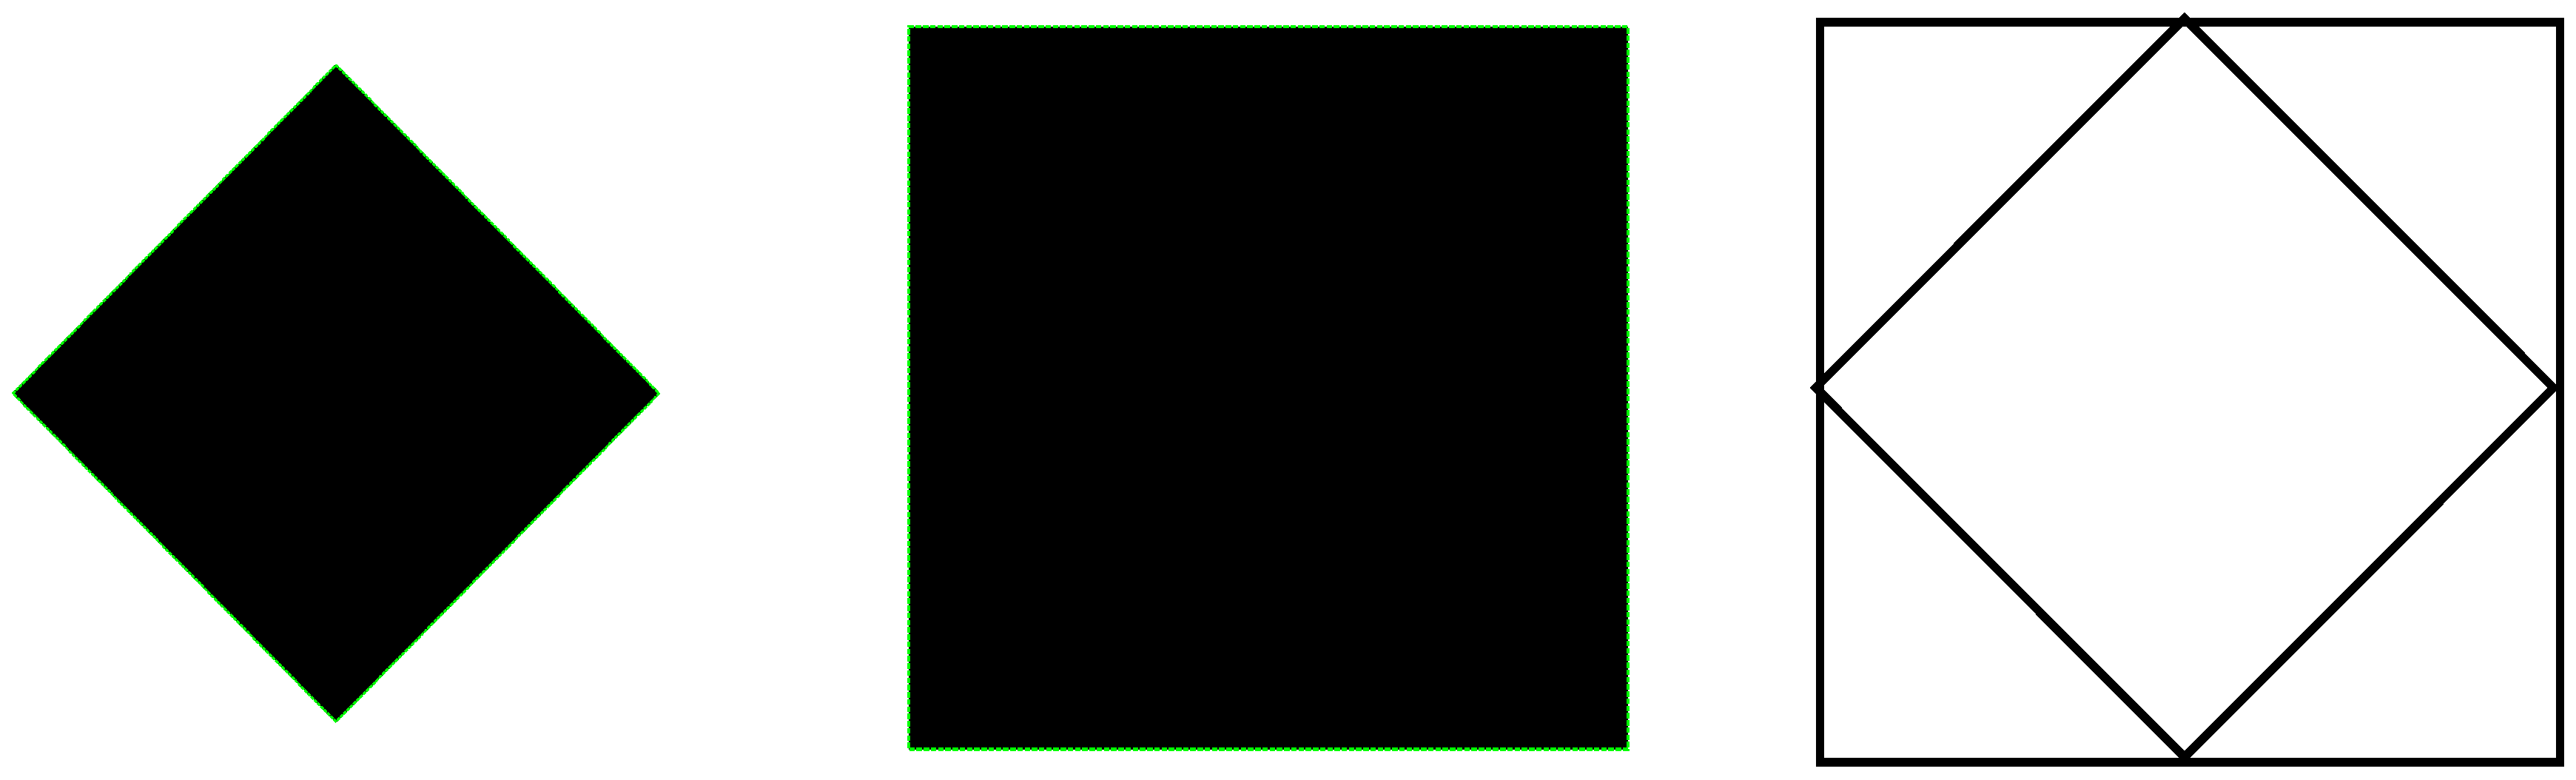
\includegraphics[width=0.7\textwidth]{SymmetrySpace}
    \caption{Two invariant Shapes, Combination is also invariant}
    \label{fig:SymmetrySpace}
\end{center}
\end{figure}





\subsection{Lie Group and Differential Equation}
For Physically-based animation,
Motions are usually described by differential equations.
Physically possible motion is the solution of the equation.
A symmetry group of a differential equation can transform solutions to other solutions.
This property helps to reduce the computational burden needed by dynamic \cms.
Lie Group Theory is introduced for this purpose.




Simply put, Lie Group is continuous group, which is also a manifold.
By the property of manifold, we can assign coordinate system and parameterize the group elements.
For example,the symmetry rotation group of square is discrete,while symmetry group of circle is continuous.
this continuous group can be parameterize by the the rotation angle.
In our discussion, for each group element $g$, $\ep$ is the parameter.

A Lie Group originates from study of differential equations.
From the algebraic perspective, the symmetrical group will keep the differential equation invariant.

For a differential equation in Equation~\ref{eq:difforg}.
\begin{equation}
\label{eq:difforg}
\dot{\state}=F(\state)
\end{equation}
Invariant function $I$ can be defined as:
\[
I(t,\state,\dot{\state})=F(\state)-\dot{\state}
\]
Solutions satisfy $I(t,\state,\dot{\state})=0$.
For the symmetry group with transformation as 
\[
(t,\state,\dot{\state}) \mapsto (\tilde{t},\tilde{\state},\dot{\tilde{\state}})
\]
We have
\[
I(t,\state,\dot{\state})=I(\tilde{t},\tilde{\state},\dot{\tilde{\state}}=0)
\]

Keep differential equations in the original form, we define the group action 
\[
g(\state)=\tilde{\state}
\]
and the \emph{lift action} 
\[
Tg(\dot{\state})=\dot{\tilde{\state}}
\]

$Tg$ can be worked out by checking the derivatives.
For the translation $g_{\ep}$ 
\[
(x,y)\mapsto (x+\ep,y+\ep)
\]
$Tg_{\ep}$ is
\[
(\dot{x},\dot{y}) \mapsto (\dot{x},\dot{y})
\]
$Tg$ is the identity element $e$.


Then $g$ transform Equation~\ref{eq:difforg} into Equation~\ref{eq:trdiff}
\begin{equation}
\label{eq:trdiff}
Tg(\dot{\state})=F(g(\state))
\end{equation}
if $g$ is symmetrical, Equation~\ref{eq:difforg} and Equation~\ref{eq:trdiff} are equivalent







 	
For the mass spring system Equation~\ref{eq:stateform}, we apply the group action 
\[
\tilde{\state}=g_{\ep}(\state)=[\ep q, \ep \qd ]
\]
then the lift action is
\[
\tilde{\state}=Tg_{\ep}(\state)=[\ep \qd, \ep \ddot{q}]
\]



by substitution $\state \mapsto \tilde{\state}$, the original system become
\[ 
\dot{\tilde{\state}}=
\left[ 
\begin{array}{cc}
0 &1\\
-1 &0 
\end{array}
\right]\tilde{\state}
\]
which is 
\begin{equation}
\label{eq:tranmas} 
\ep \dot{\state}=
\left[ 
\begin{array}{cc}
0 &1\\
-1 &0 
\end{array}
\right]\ep \state
\end{equation}

Equation ~\ref{eq:tranmas} is equivalent to  Equation~\ref{eq:stateform}.
If $\state(t)$ is a solution, so is $\tilde{\state}(t)$.

To verify the group property. define $*$ as:
\[
g_{\ep_1}*g_{\ep_2}(\state)=[\ep_1 \ep_2 q, \ep_1 \ep_2 \qd]
\]

The inverse is:
\[
g_{\ep}^{-1}=g_{\frac{1}{\ep}} \;\ep \in R^+
\]

\begin{mydef}
For a group $G$, the invairant function of state $I(\state)$ is called \emph{local motion invariant} of $G$. 
\end{mydef}

From mechanical perspective,  $I(\state)$ has important physical meaning. 
According  \textbf{Noether's Theorem}, each $I(\state)$ corresponds to a conservative law. 


\section{Control Symmetry}
\label{sec:control_symmetry}
Motions Adaptation might not only explore symmetry groups of natural dynamics.
In reallife, animals will execute control effort for adapt motions; alsoFor a dynamic system, working out the symmetry group might be an nontrivial task.
In \cms, it is possible the desired quantative properties is not an invariant of the natural dynamics.
For this end, \emph{Control Symmetry} is proposed.
Based on biological research foundings\citep{flash2007affine}, some simple group are assigned as the symmetry group of the motor dynamics system first.
The control effort are applied to ensure the symmetry.


Usually the natural dynamics are presented as by Euler-Lagrange Equation~\ref{eq:uncontrolled_euler_lagrange}\citep{Goldstein2002}.
\begin{equation}
\frac{d}{dt} \frac{\partial L}{\partial \qd} - \frac{\partial L}{\partial q} = 0
\label{eq:uncontrolled_euler_lagrange}
\end{equation}

Where $L=K-V$, $L$ is the lagrange, $K$ is the kinetic energy, $V$ is the potential energy,$q$ is the generalized coordinates, and $\qd$ is the generalized velocity.

From the symmetry perspective,transformed equation of $g$ is Equation~\ref{eq:liegroup_euler_lagrange}, for the control perspective, the controlled dynamics is Equation~\ref{eq:controlled_euler_lagrange}. If symmetry is perseved, the two equation should be equivalent, then symmetry control input $\ulocal$ can be caculated.
\begin{align}
\frac{d}{dt} \frac{\partial L}{\partial \dot{\tilde{q}}} - \frac{\partial L}{\partial \tilde{q} }&=0,\label{eq:liegroup_euler_lagrange}\\
\frac{d}{dt} \frac{\partial L}{\partial \qd} - \frac{\partial L}{\partial q}&=\ulocal. \label{eq:controlled_euler_lagrange}
\end{align}





The group we assigned are homogenous or affine group, this mainly because two reasons:
\begin{itemize}
\HiItem{Biological Reason} Homogenous and affine group close related to the vision system, which serve the foundation of navigation and perception.
\HiItem{Application Reason} Both the group elements and transformed equations are easy to compute, this will make planning and control  computational efficient.
\end{itemize}

Several groups are shown in below:

\subsection*{ Offset Action}
The offset action wil modify the coordinate by a constant, speed and time will be unchanged.
\[
(t,q,\qd) \mapsto (t,q+\ep,\qd)
\]
The state transformation and lift action are
\begin{align}
\goff(\state) &= [q+\ep,\qd] \\
T\goff(\dot{\state})&=\dot{\state}=[\qd,\qdd]
\end{align}
on phase space, if $q$ is the horizontal axis, and $\dot{q}$ is the vertical axis, offset the effect of moving the phase plot horizontally~\ref{fig:goff}.

\begin{figure}[!htbp]
  \begin{center}
      \includegraphics[width=0.7\textwidth]{g_off}
    \caption{Offset Action}
    \label{fig:goff}
\end{center}
\end{figure}

Substitued the transformed $q$ and $\qd$ into Equation~\ref{eq:liegroup_euler_lagrange} and Equation~\ref{eq:controlled_euler_lagrange}.
The symmetry control input
\begin{equation}
\ulocal(q) = \frac{\partial}{\partial q} \left(V(q)-V(\tilde{q}) \right).
\end{equation}

For example, the transformed equation and control equation are as follows.
\begin{align}
\ddot{\tilde{q}}+\tilde{q}-\ep&=0 \nonumber \\
\ddot{q}+q&=\ulocal \nonumber
\end{align}

The local control input is
\[
\ulocal(q)=\ep
\]




\subsection*{Time Scalling}

%g_st(q,dot{q})=(q,st*dot{q})
Time scaling will scale down the time variable, coordinates are kept. speed are scale up.

\[
(t,q,\qd) \mapsto (\frac{t}{\ep},q,\ep \qd)
\]

The correspond state transformation and lift action are
\begin{align}
\gts(\state)&=[q,\ep \qd] \nonumber \\
T\gts(\dot{\state})&=[\ep \qd,\ep^2 \ddot{q}]\nonumber
\end{align}

Then the local control is 
\begin{equation}
\ulocal(q) = (1-\ep^2) \frac{\partial V(q)}{\partial q}.
\end{equation}

For example, for the mass spring system,transformed and controlled equations are

\begin{align}
\frac{\ddot{\tilde{q}}}{\ep^2}+q&=0 \nonumber \\
\ddot{q}+q&=\ulocal \nonumber
\end{align}
The local control input is:
\[
\ulocal=(1-\ep^2)q
\]

\begin{figure}[!htbp]
  \begin{center}
    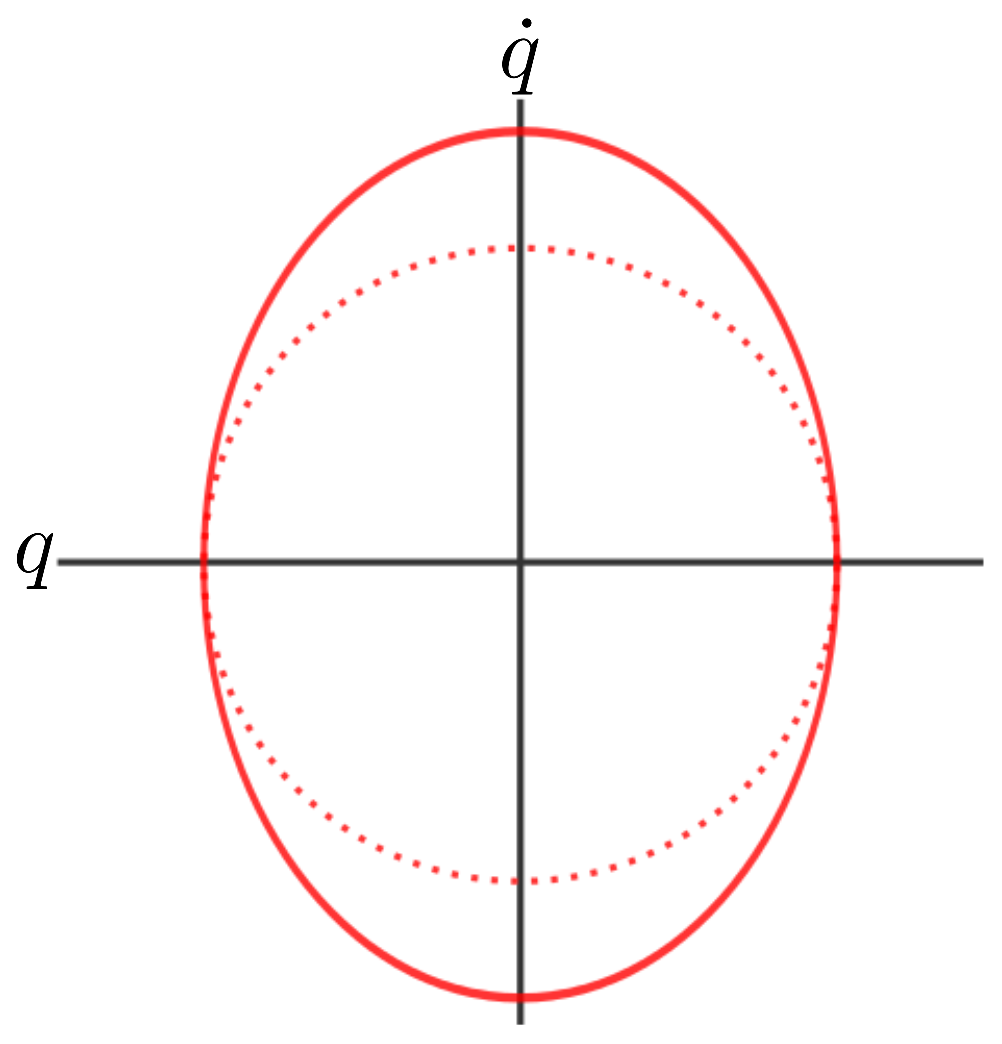
\includegraphics[width=0.7\textwidth]{g_ts}
	 \caption{Time Scaling Action}
    \label{fig:gts}
\end{center}
\end{figure}


\subsection*{Energy Scaling}
For some system moving the the conservative field.
The energy is preserved and different motion present different level of energy.
For such system, we have the energy $E(\state)=K+V$, where $K$ is the kinetic energy,
$V$ is the potential energy.
\[
E(\tilde{\state})=\ep^2 E(x)
\]
To generalize uniformlly
\begin{align}
K(\tilde{\state})=\ep^2 K(\state) \nonumber\\
V(\tilde{\state})=\ep^2 V(\state) \nonumber
\end{align}


If the mass of system is constant, energy scaling can be achieved by linear transformation.
\[
(t,q,\qd ) \mapsto ( \frac{f(\ep)}{\ep}t ,f(\ep)q,\ep\qd)
\]
$f(\ep)$ is a function of $\ep$, which is determined by the consevative force.
On phase plot, this has the effect enlarge the phase portrait,as show in Figure~\ref{fig:gen}.
\begin{figure}[!htbp]
  \begin{center}
      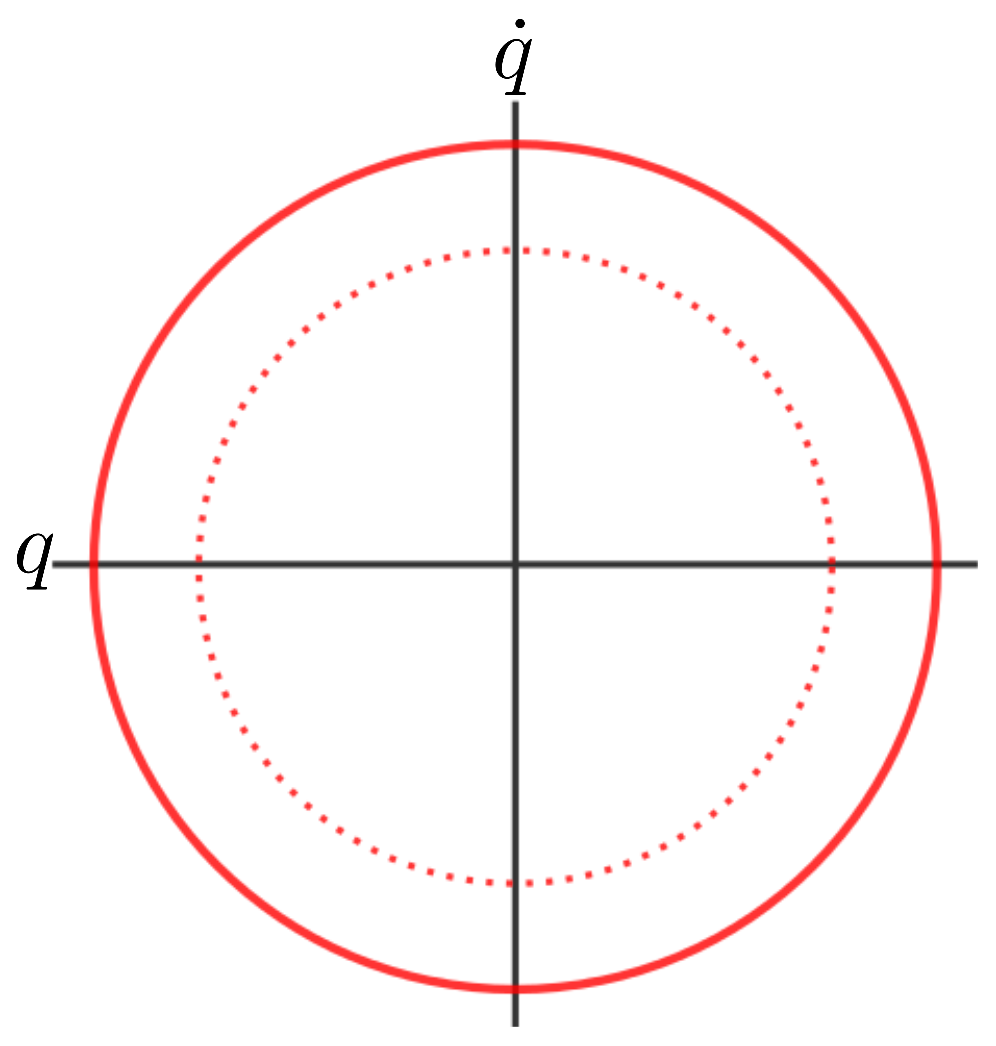
\includegraphics[width=0.7\textwidth]{g_en}
    \caption{Energe Scaling Action}
    \label{fig:gen}
\end{center}
\end{figure}

The state transformation and lift action
\begin{align}
\gen(\state)&=(f(\ep) q,\ep \dot{q}) \nonumber\\
T\gen(\dot{\state})&=(\ep \dot{q},\frac{\ep^2}{f(\ep)}\qdd)
\end{align}
$\ulocal$ can be developed by applying the pos scaling and time scaling in a combined manner.



For the mass spring system , $E=\frac{1}{2}(q^2+\qd^2)$,$f(\ep)=\ep$, and because the energy scaling is kept by the original system, we have
\[
\ulocal=0
\]



\subsection*{Time Offset}
we can also offset the time $t$
\[
(t,q,\qd) \mapsto (t+\ep,q,\qd)
\]

For dynamic system, Time offset symmetry is preserved by any system.
For system with limit cycle, Time offset has a special effects like phase modification.
On phase plot, this has the effect rotate on the limit circle about an angle, as shown in Figure~\ref{fig:gtoff}.
\begin{figure}
  \begin{center}
      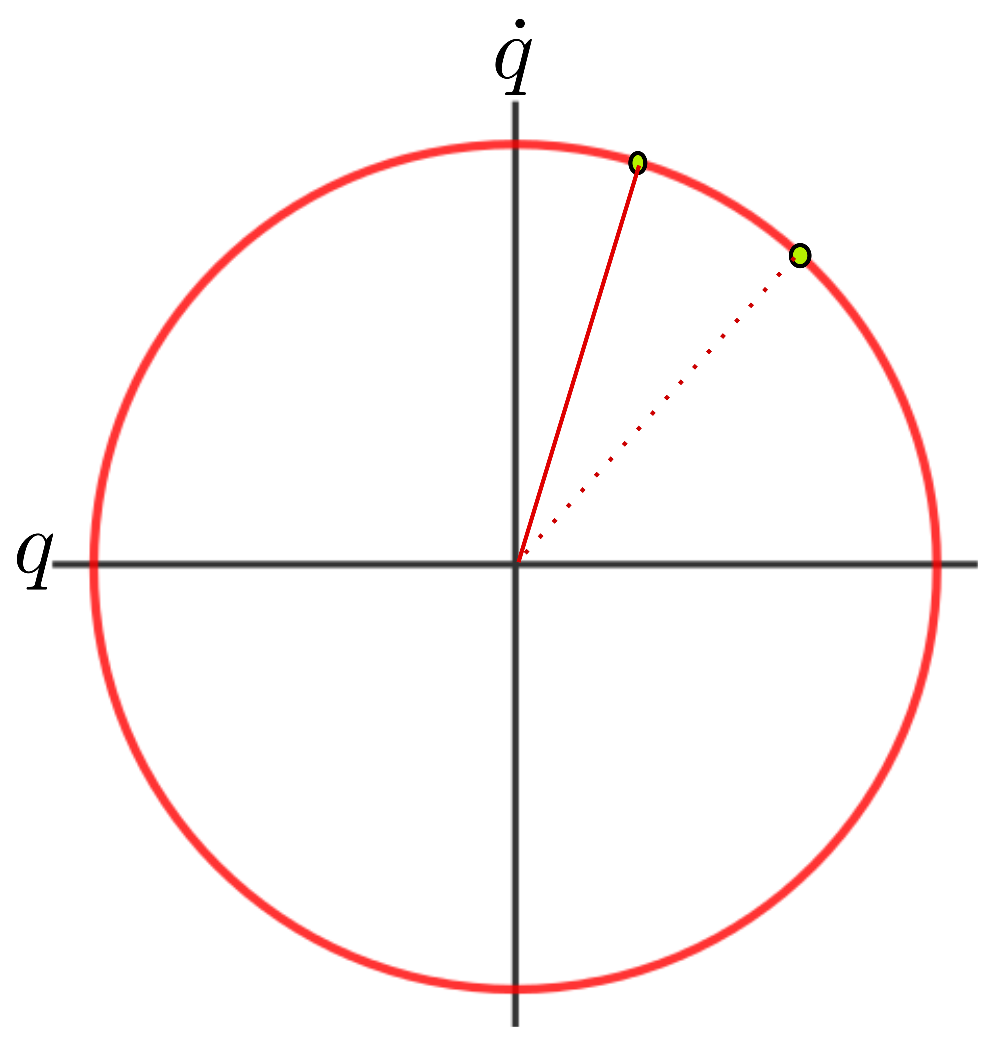
\includegraphics[width=0.7\textwidth]{g_toff}
    \caption{Offset Action}
    \label{fig:gtoff}
\end{center}
\end{figure}





\section{Example:Bouncing Ball dropt from Different Height}
Even it is a hybrid system,
The bouncing ball system has a energy scaling symmetry.

the energy function 
\[
E=\mathrm{g}q+\frac{1}{2}m\qd^2
\]
then
\[
f(\ep)=\ep^2
\]
the energy scaling transformation is
\[
\gen(\state)=[\ep^2 q, \ep \qd]
\]

Given the motion of a ball dropt at $5$,shown in Figure~\ref{fig:bouncing5},set $\ep=\sqrt{2}$, through transformation, motion droped from $10$ are shown in Figure~\ref{fig:bouncing10}
\begin{figure}[!htbp]
  \begin{center}
      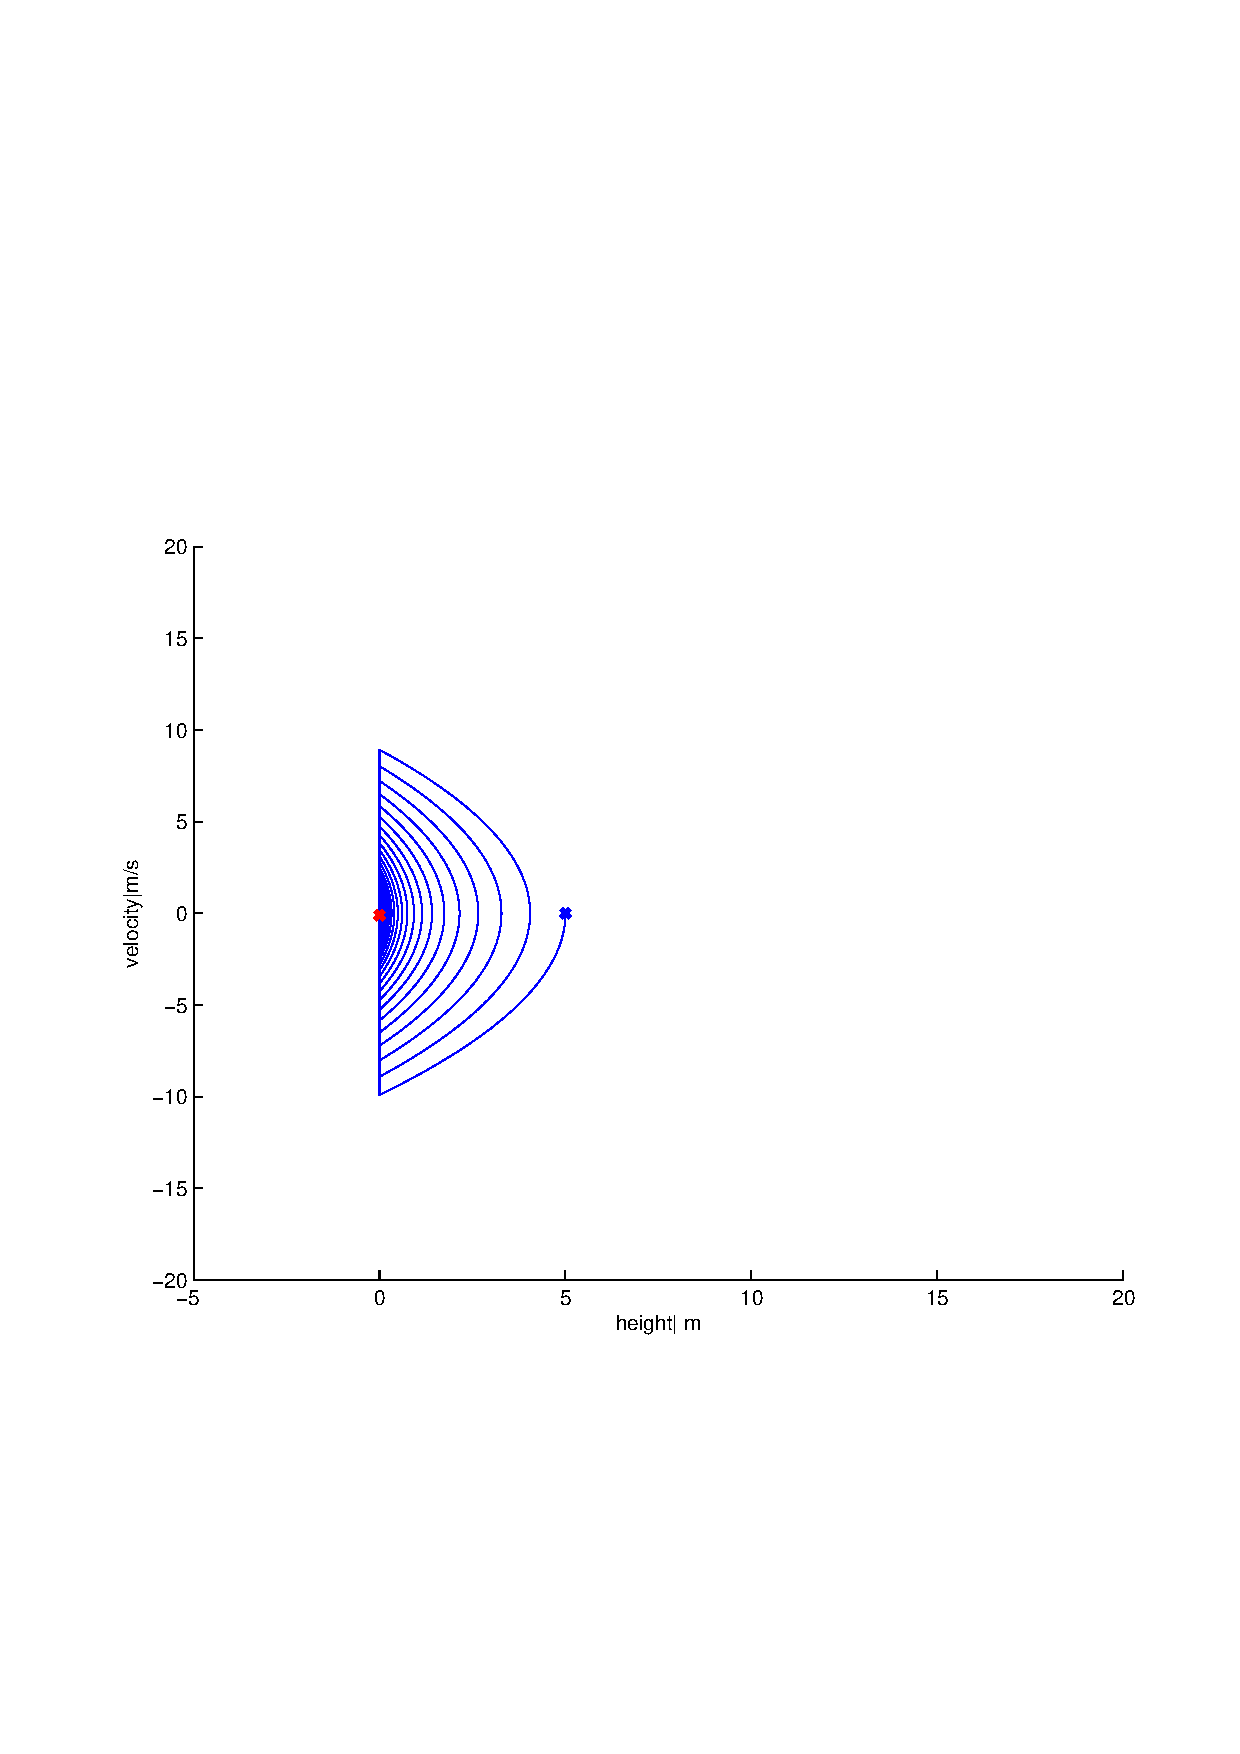
\includegraphics[width=0.7\textwidth]{BouncingBallPhasePlotuncontrolledDropAt5}
    \caption{Drop at 5}
    \label{fig:bouncing5}
\end{center}
\end{figure}


\begin{figure}[!htbp]
  \begin{center}
      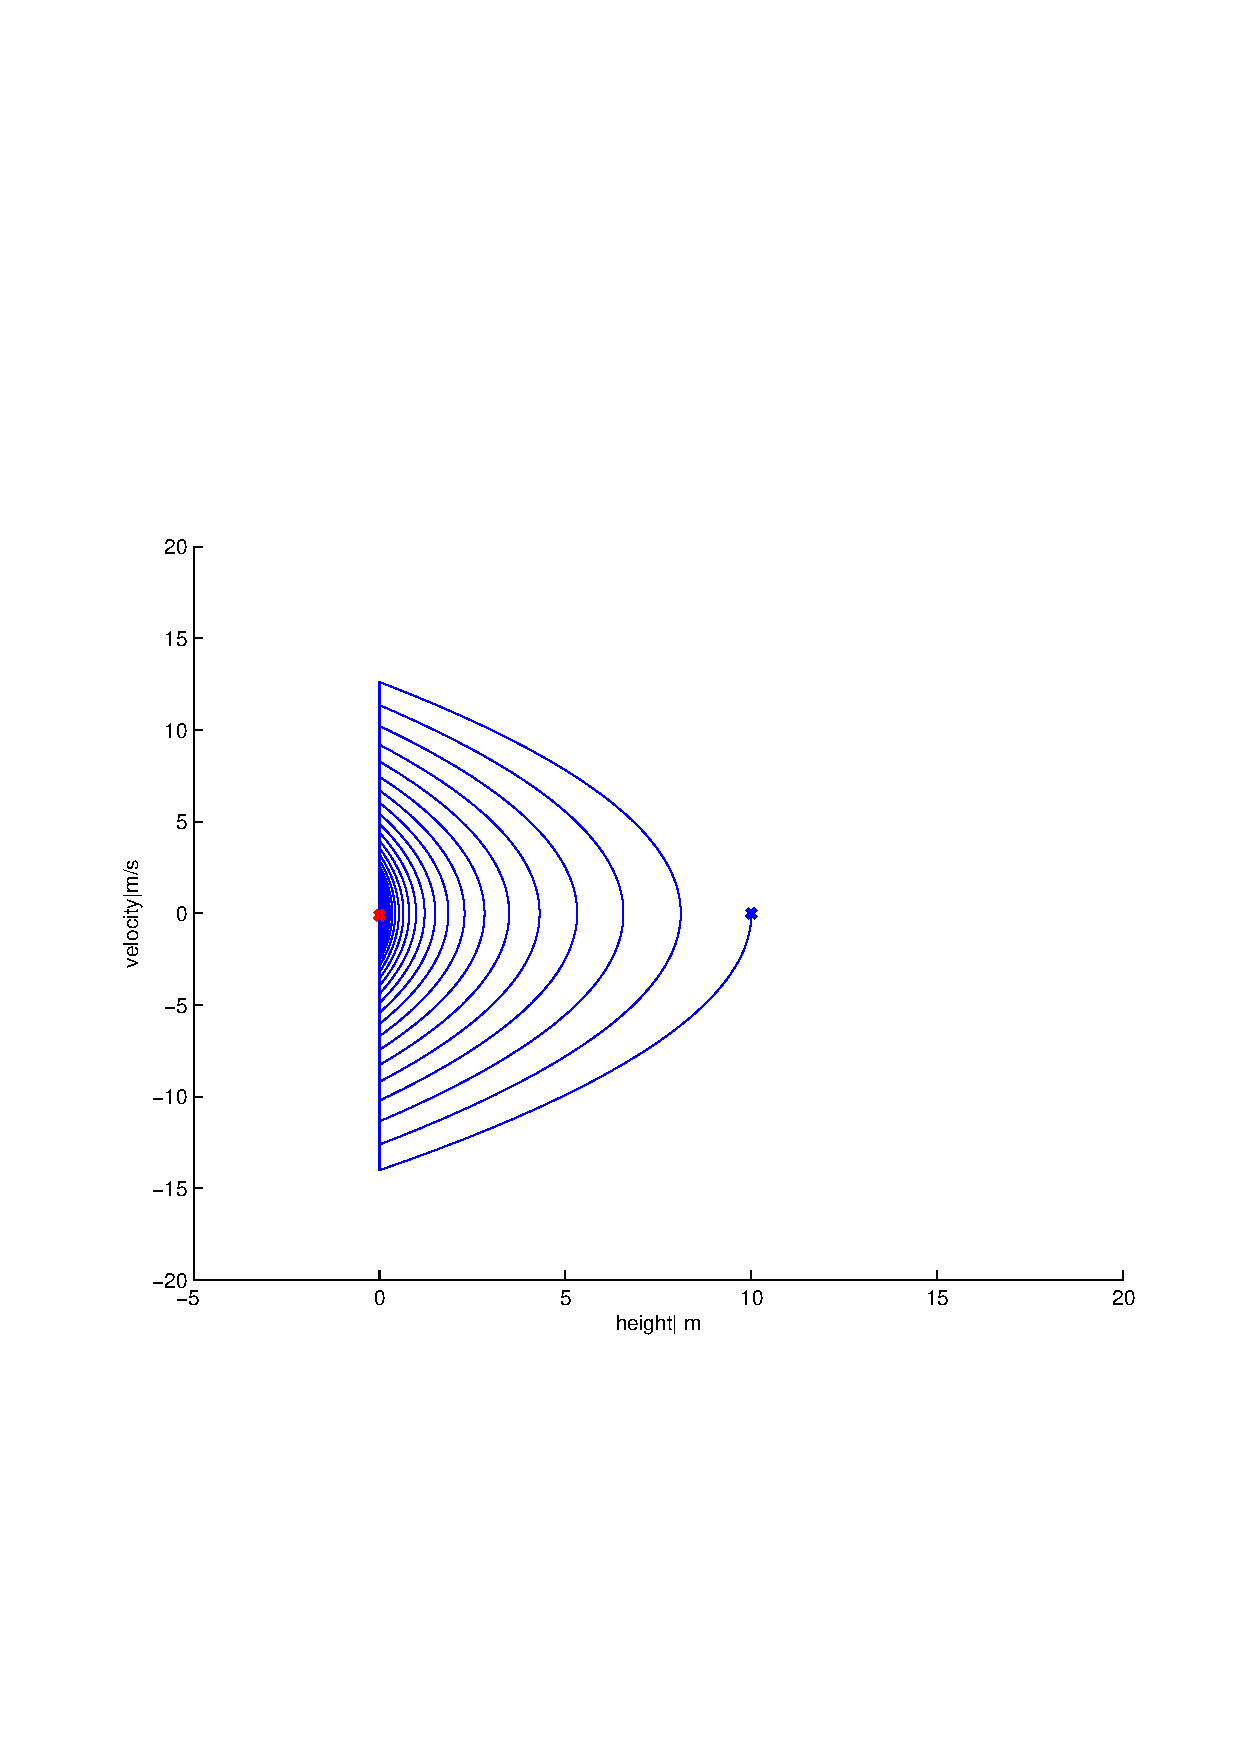
\includegraphics[width=0.7\textwidth]{BouncingBallPhasePlotuncontrolledDropAt10}
    \caption{Drop at 10}
    \label{fig:bouncing10}
\end{center}
\end{figure}




